\documentclass[../improvements.tex]{subflies}

\begin{document}
  プロセッサが動的分岐予測機能をもっているなら, 分岐が原因でパイプラインがフラッシュされた時に
  失われるクロックサイクル数を減らすことができる.
  この章では, 今回の設計において動的分岐予測の実装方法と評価結果について述べる.

  \subsubsection{分岐予測の対象命令}
  分岐予測の対象命令を, 無条件分岐命令と条件付き分岐命令 
  (それぞれ表 \ref{table:isa} にある J形式と B形式の命令) とする.
  無条件分岐命令は必ず分岐するので, 条件付き分岐命令よりも予測しやすいため, 
  分岐予測の対象に含めることにした.

  \subsubsection{予測方法}
  無条件分岐命令と条件付き分岐命令の予測しやすさに違いがあるため, 
  命令ごとに予測できるローカル予測器を採用した.
  実装では, エントリー数が 32 の参照テーブル (図 \ref{fig:predictor-table}) を用意した.
  命令の下位2ビットは常に \verb|00| であるため, 
  参照テーブルのエントリーは, 対象命令の 6ビット目から 2ビット目までの値で指定する.
  そして, 1つのエントリーに $2[bit]$ の状態信号と $32[bit]$ の分岐先アドレスを保持する.
  状態信号の値と分岐方向の予測を表 \ref{table:predictor-state} に示す.
  
  % TODO: This figure don't have to be this big because it's not that important
  \begin{figure*}
    \resizebox{2\columnwidth}{!}{
      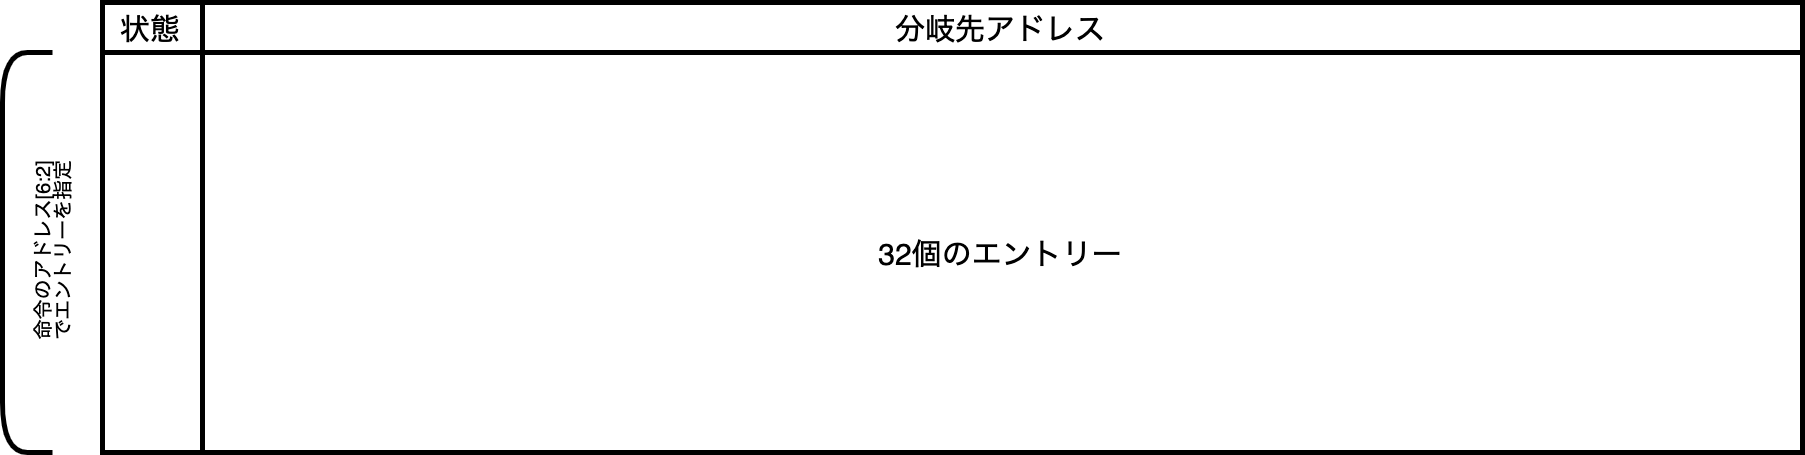
\includegraphics{../../images/predictor_table.png}
    }
    \caption{予測器の参照テーブル}
    \label{fig:predictor-table}
  \end{figure*}

  \begin{table}[h!]
    \centering
    \begin{tabular}{|l|l|}
    \hline
    状態信号 & 分岐方向の予測 \\ \hline
    00 (STRONG\_NOT\_TAKE) & 分岐しない \\
    01 (WEAK\_NOT\_TAKE) & 分岐しない \\
    10 (WEAK\_TAKE) & 分岐する \\
    11 (STRONG\_TAKE) & 分岐する \\ \hline
    \end{tabular}
    \caption{予測器の状態信号と分岐方向の予測}
    \label{table:predictor-state}
  \end{table}

  命令メモリからフェッチした命令が予測の対象命令である時に, 
  参照テーブルのエントリーの状態信号と分岐先アドレスを元に, 
  分岐方向と分岐先アドレスをそれぞれ予測する.
  また, 予測の対象命令ではない時に, 「分岐しない」と予測する.

  \subsubsection{予測が間違えた時の処理}
  分岐方向の予測, または分岐先アドレスの予測が間違えた場合, 
  PC を ALU で計算された正しい分岐先アドレスへと更新し, 
  予測器の参照テーブルの更新を行う.
  参照テーブルの該当エントリーに対して, 
  状態信号の更新を図 \ref{fig:predictor-state-transition} のように行い, 
  分岐先アドレスを ALU で計算された分岐先アドレスへ更新する.

  \begin{figure*}
    \centering
    \resizebox{1.5\columnwidth}{!}{
      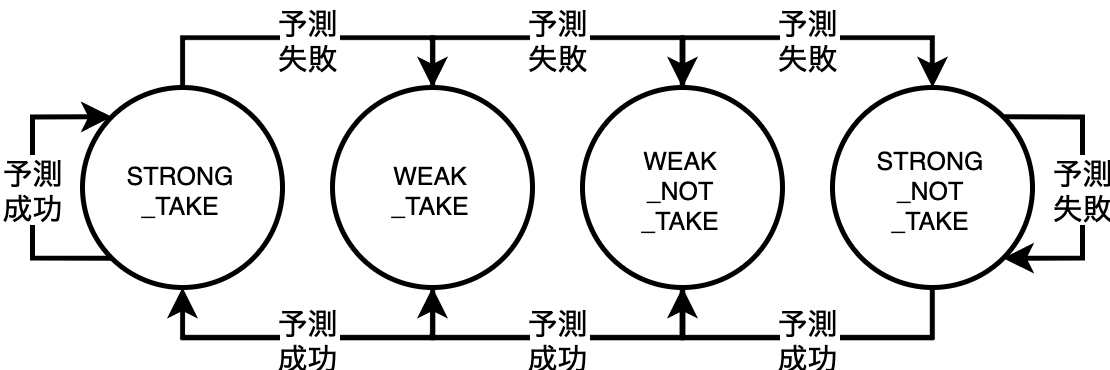
\includegraphics{../../images/predictor-state-transition.png}
    }
    \caption{$2[bit]$ 予測器: 状態遷移図}
    \label{fig:predictor-state-transition}
  \end{figure*}

  \subsubsection{分岐予測の評価と論理合成}
  エントリー数が 32個の参照テーブルをもつ分岐予測器を, 
  MiBench ベンチマークプログラムで実行クロックサイクル数とミス率を測定し, 論理合成を行った.
  実行クロックサイクル数の結果を表 \ref{table:mibench-improved} に, 
  ミス率の結果を表 \ref{table:miss-rate} に, 
  論理合成の結果を表 \ref{table:logic-synthesis-improved} にまとめる.

  \begin{table*}[bp]
    \centering
    \begin{tabular}{|c|r|r|}
      \hline
      ベンチマークプログラム & \multicolumn{1}{c|}{\begin{tabular}[c]{@{}c@{}}クロックサイクル数\\ (分岐予測実装前)\end{tabular}} & \multicolumn{1}{c|}{\begin{tabular}[c]{@{}c@{}}クロックサイクル数\\ (分岐予測実装後)\end{tabular}} \\ \hline
      stringsearch & 10594 & 6966 \\
      bitcnts & 56040 & 44680 \\
      dijkstra & 4079473 & 3048011 \\ \hline
    \end{tabular}
    \caption{分岐予測実装前後のプログラム実行クロックサイクル数}
    \label{table:mibench-improved}
  \end{table*}

  \begin{table*}[]
    \centering
    \begin{tabular}{|c|r|r|r|}
    \hline
    ベンチマークプログラム & \multicolumn{1}{c|}{分岐予測対象命令数} & \multicolumn{1}{c|}{予測失敗命令数} & \multicolumn{1}{c|}{予測失敗率 {[}\%{]}} \\ \hline
    stringsearch & 2113 & 131 & 6.20 \\
    bitcnts & 9930 & 690 & 6.95 \\
    dijkstra & 869932 & 12886 & 1.48 \\ \hline
    \end{tabular}
    \caption{分岐予測の予測失敗率}
    \label{table:miss-rate}
  \end{table*}

  参照テーブルのエントリー数を変化させて評価を行ったが, 
  32個以上の参照テーブルをもつ場合の論理合成にかかる時間が長かったため, 
  32個のエントリーを選んだ.

  \subsubsection{更に改善できる点}
  今回の分岐予測の参照テーブルの実装方法であれば, 
  シミュレーション上でしか, 正確な結果, または, 報告した通りの性能向上が出せない可能性がある.
  シミュレーションの環境において, あるエントリーの状態信号が初期化されていない時, 
  その信号は \verb|00|, \verb|01|, \verb|10|, \verb|11| のどれでもなく, \verb|xx| である.
  ただし, Verilog-HDL で $2[bit]$ の条件文をもつ \verb|case| 分を使えば, 
  \verb|default| で \verb|xx| の信号に対する処理ができる.
  今回の実装において, この \verb|case| 分の \verb|default| で
  予測を \verb|WEAK_NOT_TAKEN| と出力するように記述している.
  しかし, 実機では \verb|xx| の信号が存在しないため, 
  この実装が実機上どんな動作をするかがわからない.
  エントリー数が 32 個以上の参照テーブルを実装すれば, 
  参照テーブルがメモリとして論理合成され, 
  プロセッサのリセット時に全てのエントリーを 0 にリセットすることが現実的ではなくなる.
  そのため, 参照テーブルの実装方法を変えるか, 参照テーブルを使わない実装方法に変える必要がある.

\end{document}
